\section{Autonomous Technologies}
Autonomous Technologies are solutions powered by AI or self-intelligence. A system is said to be "autonomous" if it is capable of sensing and acting on stimuli without human intervention. They are an off-shoot of the larger domain of Robots and Robotics. 
\\ 

Robots, however, are a modern concept in man's psyche. Robots were not yet part of popular science fiction until 1917, when Joseph Capek wrote the short story Opilec describing automats and in 1921, when his brother Karel Capek wrote the play Rossum’s Univeral Robots (RUR) - a play to evoke a sense of protest against the rapid growth of modern technology by describing the evolution of robots with increasing capabilities and the eventual revolt of these robots against their human counterparts. It is not known which brother came up with the term robot, and apparently, it is a matter of debate in the Czech literary world. Ever since then, the concept of robots has been reinforced in our memory palace through countless examples in pop culture and media. However, what began as far-fetched pipe dreams from the novels of Isaac Asimov are now gradually becoming a part of our everyday lives. From robotic vacuum cleaners to robot hotel receptionists, Robots are quickly becoming a part of our everyday lives. \cite{hockstein2007history}. 
\begin{figure}[H]
    \centering
    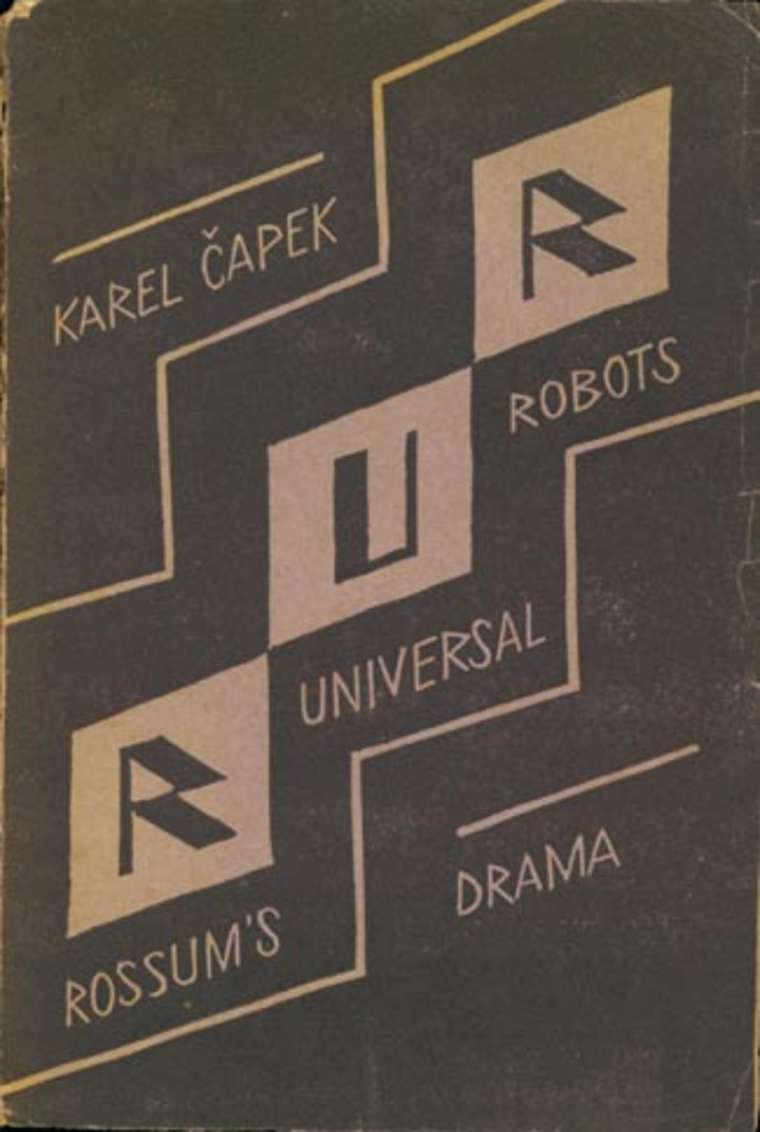
\includegraphics[width=\textwidth,height=7cm,keepaspectratio=true]{src/Images/Rosumovi_Univerzální_Roboti_1920.jpg}
    \caption{
     Cover of Karel Capek's Rossum’s Univeral Robots (RUR) \cite{rur_img}  
    }
\end{figure}
\\

The economy experienced a boom after World War 2, leading to advances in electronic components such as portable radios, transistors, digital logic, servers, and more. These paved the way for research and progress in robotics. Initially, the industrial sector showed interest in robotics to perform jobs that were too dangerous for humans. The first commercially developed industrial robot was "Ultimate," a type of industrial arm created by George C. Devol in 1961. It was sold to a General Motors plant to remove high-temperature parts from the die-cast. Since then, robots have found further applications in domains such as manufacturing, mining, agriculture, medicine, and more. \cite{stone2018history}. Robotics and artificial intelligence have also influenced the field of autonomous automotive technologies such as Self-driving Cars, Autonomous Surface Vessels (ASV), and Unmanned Aerial Vehicles (UAV). 
\\

The history and technology behind autonomous driving technologies go back to the early 20th century, in 1926, it was called the Linriccan Wonder, a remote-control car, which received commands to control its electric motors connected to breakers to control its motion. In the coming decades, other work, such as an electric car powered by circuits by Normal Bel Geddes and an autonomous car controlled based on a pattern of wires by RCA labs and General Motors, also heavily influenced the early years of autonomous driving technologies. \cite{divakarla2019review}. In the 1960s, General Motors worked with Leland Hancock and L.N. Ress to develop an idea for semi-autonomous vehicles. Together, they took the idea to the actual road and launched a series of experimental vehicles called Firebird. The Firebird was showcased at the General Motors Auto show called Motorama. \cite{kroger2016automated}. Recently, the big players in the self-driving scene are Google's Waymo (Or technically, its parent company, Alphabet), GM's Cruise, and XooX and, in China, Baidu. Google currently offers paid rides on their robo-taxis in San Francisco and Cruise is expanding to over 10 cities in 2024 for testing and potential future commercial operations. 
\begin{figure}[H]
    \centering
    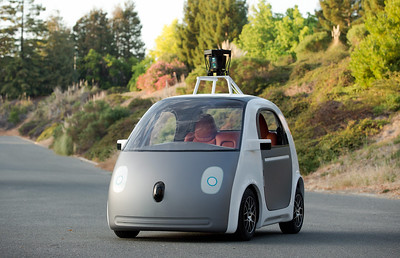
\includegraphics[width=\textwidth,height=5cm,keepaspectratio=true]{src/Images/waymo_car.jpg}
    \caption{
      An early version of Waymo's self-driving car concept. \cite{waymo_img}
    }
\end{figure}
\\
However, the adoption of autonomous technologies has been slower than promised due to the depth of the technical and regulatory challenges, and since the 1970s, there has been a parallel effort from the automotive industry to develop and adopt ADAS (Advanced Driver Assistance System) solutions such as ABS (Anti-lock braking system), Blind spot monitoring, backup sensors and cameras, lane-keep assist, due to more commercial interest from consumers and more accessible barrier to entry into different regulatory markets. \cite{okuda2014survey}
\begin{figure}[H]
    \centering
    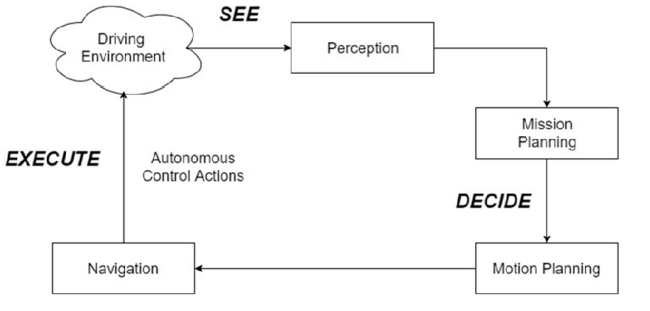
\includegraphics[width=\textwidth,height=5cm,keepaspectratio=true]{src/Images/adas.PNG}
    \caption{
      High level ADAS Architecture \cite{pereira2012integrated}
    }
\end{figure}
\\
Today, built on top of the previous research and experience in vehicle dynamics, ADAS, breakthroughs in AI - particularly in Computer Vision through deep learning, AI acceleration hardware such as GPU, and broader market availability of new sensing solutions such as Lidar and millimeter wave Radar have empowered self-driving research and industry application further to a point where they are becoming safer and commercially available. 
\cite{okuda2014survey}
\begin{figure}[H]
    \centering
    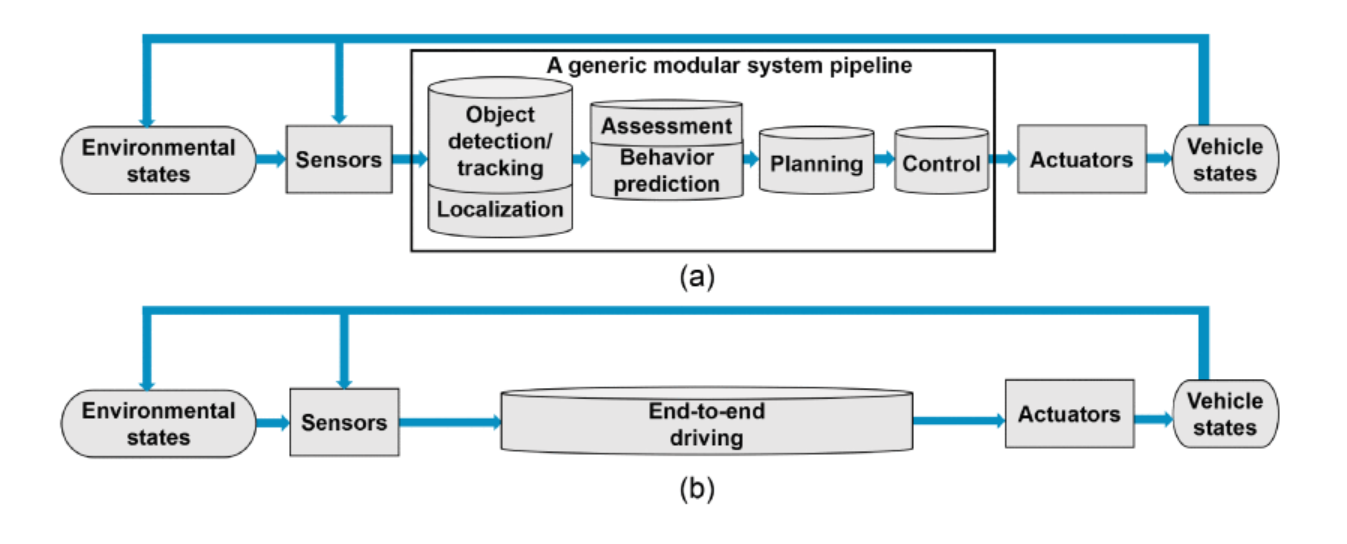
\includegraphics[width=\textwidth,height=7cm,keepaspectratio=true]{src/Images/auv_img.PNG}
    \caption{
      High level flow of execution in an autonomous driving vehicle \cite{okuda2014survey}
    }
\end{figure}
\\

Figure 1.9 illustrates the standard components and the flow of data or execution among them. The sensors used in autonomous vehicles are mono or stereo cameras, mmw radars, and lidars. The choice of sensing solution depends on various factors, such as the cost of the final product, operating environments, and the selected autonomy tech stack. Lower-cost end products, such as smaller cars, usually employ cheaper sensing solutions, such as cameras and automotive-grade radars. However, with increasing demand for autonomous vehicles and given the scale of the automotive industry, lidars are becoming more commercially available and less expensive. \cite{okuda2014survey}. Manufacturers like Tesla are employing camera-only autonomous solutions based on their findings and experience. Still, companies like Cruise and Waymo are opting for more sophisticated solutions comprising cameras and lidars. When choosing any sensing solution, high sensor redundancy is of the utmost importance for robustness and reliability.
\cite{okuda2014survey}
\begin{figure}[H]
    \centering
    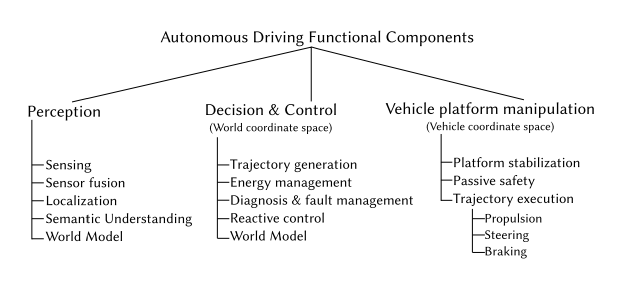
\includegraphics[width=\textwidth,height=7cm,keepaspectratio=true]{src/Images/auv_comp.PNG}
    \caption{
      Components of "Sense, Think and Act" Paradigm of autonomous driving \cite{behere2015functional}
    }
\end{figure}
\\
 The sensing task is usually combined with perception or "Sense" operations such as Object detection, Scene segmentation, Sensor Fusion, Localization, and Mapping. Sensor fusion involves combining data from multiple sensors or sensor modalities. For example, Camera-Radar sensor fusion detects and tracks objects simultaneously in both sensor modalities. Mapping is the process of building a map of the environment using combined sensor input. Localization is the task of localizing the robot on a map using the sensor input. Together,  mapping and localization can be combined into one continuous process called Simultaneous Localization and Mapping. The produced map, along with the robot's position, is fed to the "Think" or planning portion of the system, like the path planner, to produce velocity commands and trajectory for the controller unit to execute, dynamically updating the world-state based on actions taken, etc. The "Act" portion of the autonomous vehicle usually consists of a controller that can directly/indirectly control the movements of the vehicle's actuators. \cite{behere2015functional}
 \begin{figure}[H]
    \centering
    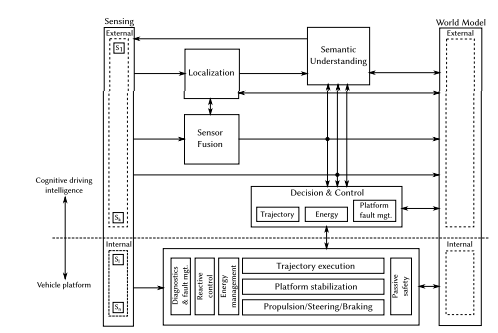
\includegraphics[width=\textwidth,height=5cm,keepaspectratio=true]{src/Images/auv_arch.PNG}
    \caption{
      Functional Architecture of a Self-driving vehicle \cite{behere2015functional}
    }
\end{figure}
\\